
\documentclass{amsart}


\usepackage{graphicx}
\graphicspath{ {Images/} }
\usepackage[section]{placeins}
\usepackage{amsfonts}
\usepackage{amsmath}
\usepackage{amscd}
%\usepackage{xy}
\usepackage{amssymb}
\usepackage{verbatim}
\usepackage{hyperref}
\usepackage{txfonts}
\usepackage{float}
\usepackage[nottoc]{tocbibind} %Adds "References" to the table of contents


\newenvironment{proof*}{\noindent\emph{Proof}}{$\square$\smallskip}


\newtheorem{theorem}{Theorem}[section]
\newtheorem{problem}[theorem]{Problem}
\newtheorem{Definition}[theorem]{Definition}
\newtheorem{lemma}[theorem]{Lemma}
\newtheorem{Example}[theorem]{Example}
\newtheorem{corollary}[theorem]{Corollary}
\newtheorem{Remark}[theorem]{Remark}
\newtheorem{proposition}[theorem]{Proposition}
\newtheorem{conjecture}[theorem]{Conjecture}
\newtheorem{fact}[theorem]{Fact}
\newtheorem{claim}[theorem]{Claim}
\newtheorem{question}[theorem]{Question}
\newtheorem{fig}[theorem]{Figure}
\newtheorem{Exercise}[theorem]{Exercise}
\newtheorem{Exercises}[theorem]{Exercises}
\newtheorem{Notation}[theorem]{Notation}
\newtheorem{Convention}[theorem]{Convention}
\newtheorem{hypothesis}[theorem]{Hypothesis}

%These new environments eliminate italics from definitions, examples, remarks, exercises.
\newenvironment{definition}{\begin{Definition}\normalfont}{\end{Definition}}
\newenvironment{example}{\begin{Example}\normalfont}{\end{Example}}
\newenvironment{remark}{\begin{Remark}\normalfont}{\end{Remark}}
\newenvironment{exercise}{\begin{Exercise}\normalfont}{\end{Exercise}}
\newenvironment{exercises}{\begin{Exercises}\normalfont}{\end{Exercises}}
\newenvironment{notation}{\begin{Notation}\normalfont}{\end{Notation}}
\newenvironment{convention}{\begin{Convention}\normalfont}{\end{Convention}}

%Definitions that I'll probably want in most papers:
\newcommand{\br}{\ensuremath{\mathbb{R}}} %The real numbers
\newcommand{\bz}{\ensuremath{\mathbb{Z}}} %The integers
\newcommand{\bn}{\ensuremath{\mathbb{N}}} %The natural numbers
\newcommand{\bc}{\ensuremath{\mathbb{C}}} %The complex numbers
\newcommand{\bq}{\ensuremath{\mathbb{Q}}} %The rational numbers
\newcommand{\id}{\ensuremath{\mathrm{id}}} %The identity morphism
\newcommand{\incl}{\ensuremath{\mathrm{incl}}} %The inclusion morphism
\newcommand{\bm}{\ensuremath{\mathbb{M}}} %The m for matrix algebra
\newcommand{\diam}{\ensuremath{\mathrm{diam}}} %The diameter
\newcommand{\e}{\ensuremath{\mathrm{e}}} %The number e
\newcommand{\image}{\ensuremath{\mathrm{im}}} %The image of a map

%Defintions that are specific to another paper (or series of papers):
%\newcommand{\lig}{\text{$\Cal G_{LI}(X)$}} %Notation for the local isometry groupoid of X
\newcommand{\ligx}{\ensuremath{\mathcal{G}_{LI}(X)}} %Better name for notation for the local isometry groupoid of X
\newcommand{\lsgx}{\ensuremath{\mathcal{G}_{LS}(X)}} %Notation for the local similarity groupoid of X
\newcommand{\symtv}{\ensuremath{Sym_\infty(T,v)}} %Notation for the symmetry group at infinity of (T,v)
\newcommand{\plix}{\ensuremath{\mathcal{P}_{LI}(X)}} %Notation for the pseudogroup of local isometries on X
\newcommand{\eligx}{\ensuremath{{\mathcal{G}}^{\epsilon}_{LI}(X)}} %Notation for the epsilon local isometry groupoid of X
\newcommand{\eiligx}{\ensuremath{{\mathcal{G}}^{\epsilon_i}_{LI}(X)}} %Notation for the epsilon_i local isometry groupoid of X
\newcommand{\eioligx}{\ensuremath{{\mathcal{G}}^{\epsilon_{i+1}}_{LI}(X)}} %Notation for the epsilon_i+1 local isometry groupoid of X
\newcommand{\pgd}{\ensuremath{{\mathcal{PG}}({D},v_0)}} %Notation for the path groudoid of D based at v_0
\newcommand{\pgb}{\ensuremath{{\mathcal{PG}}({B(T,v)})}} %Notation for the path groudoid of the Bratteli diagram B(T,v)
\newcommand{\pb}{\ensuremath{{\mathcal{P}}({B(T,v)})}} %Notation for the path space of the Bratteli diagram B(T,v)
\newcommand{\gammax}{\ensuremath{\mathcal{G}_{\Gamma}(X)}} %Notation for the Gamma groupoid of X
\newcommand{\gammay}{\ensuremath{\mathcal{G}_{\Gamma}(Y)}} %Notation for the Gamma groupoid of Y
\newcommand{\g}{\ensuremath{\mathcal{G}}} %Notation for a groupoid 
\newcommand{\Cay}{\ensuremath{{\rm Cay}}} %Notation for Cayley graph
\newcommand{\co}{\ensuremath{\colon}} % colon for funnctions
\newcommand{\symdiff}{\ensuremath{,\triangle\,}} %Notatin for the triangle in a symmetric difference.


%Definitions specific to this paper "Notes on Ultrametrics"
\newcommand{\sm}{\ensuremath{{\rm Sim}}} %Notation for similarity structure
\newcommand{\Aut}{\ensuremath{{\rm Aut}}} %Notation for automorphism group
%\newcommand{\ld}{\ensuremath{{\ell_{\mathrm{dom}}}}} %Notation for domain length function
%\newcommand{\lr}{\ensuremath{{\ell_{\mathrm{ran}}}}} %Notation for range length function

%%%%%For metric book
\newcommand{\sH}{\ensuremath{\mathcal{H}}} %Notation for hyperspace

%Definitions specific to this paper "Local similarities and the Haagerup Property"
\newcommand{\bi}{\ensuremath{{\rm Bi}}} %Notation for the set of bijections

%Definitions specific to Notes with Dan Farley
\newcommand{\lk}{\ensuremath{{\rm lk}}} %Notation for link
\newcommand{\sta}{\ensuremath{{\rm st}}} %Notation for star
\newcommand{\dlk}{\ensuremath{{\lk_{\downarrow}}}} %Notation for link
\newcommand{\expa}{\ensuremath{{\rm expansion}}} %Notation expansion of a vertex
\newcommand{\depth}{\ensuremath{{\rm depth}}} %Notation depth of a vertex
                            
\title{Discrete Morse Theory and Fundamental Groups in Moduli Spaces of Planar Linkages}
\author{Dana Lee A. Lewis}
\author{Griselda Martinez}
\author{Maram F. Sultan}
\date{July 2015}
\begin{document}


\maketitle
\section{Abstract}

Following R. Forman\cite{RFOR}, G. Panina and A. Zhukova\cite{PANZU} determined a discrete gradient vector field for the moduli spaces on planar linkages. Using this discrete gradient vector field and applying the rewriting system develop by  D. Farley and L. Sabalka\cite{FS1}, we were able to compose an easier method for computing the fundamental groups of these moduli spaces.

\section{Introduction}
We consider the moduli spaces of planar polygonal n-linkages in which cells are labeled by cyclically ordered partitions of the set $[n]=\{1,\ldots,n\}$\cite{PANZU}. In their paper, G. Panina and A. Zhukova introduce a method of applying a version of R. Forman's perfect discrete Morse function on these spaces. We, however, did not develop techniques following the \emph{perfect} discrete Morse function, as our research does not utilize the \emph{path reversing technique} developed originally by R. Forman. The purpose of understanding this discrete Morse function was to assist us in efficiently computing the fundamental groups of the moduli spaces.

In order to compute the fundamental groups we adopted D. Farley and L. Sabalka's rewrite techniques. We used \textbf{Theorem 3.21} to tie together the ideas of the discrete Morse function and the fundamental groups of the moduli spaces. This theorem allowed us to represent the fundamental groups as the relations of \emph{critical cells} in the configuration spaces.

In our research we developed algorithms which simplify the rewriting of the fundamental groups and provide us the means to easily observe which \emph{redundant 1-cells} are \emph{collapsible} and which are \emph{critical}.

More specifically, Section 3 of our paper provides the background information regarding moduli spaces, cell structures, discrete Morse theory and the rewriting system. The final section of our paper presents our research and the procedures we found which shorten the act of computing fundamental groups considerably.

\section{Background}
\subsection{Moduli Spaces of Planar Polygons}
The definitions used in this section are those used by G. Panina and A. Zhukova in their work to explain the attributions of moduli spaces. 
\begin{definition}
\cite{PANZU} A \textit{polygonal n-linkage} is a sequence of positive numbers ${L} = ({l_1,...,l_n})$. It should be interpreted as a collection of rigid bars of lengths ${l_i}$ joined consecutively in a chain by revolving joints. We always assume that the triangle inequality holds, that is,
\begin{equation}
\forall j, {l_j} < \frac{1}{2} \sum_{i=1}^{n} {l_i}
\end{equation}
which guarantees that the chain of bars can close.
A \textit{planar configuration} of L is a sequence of points
\begin{equation}
P= (p_1, ... , p_n), {p_i} \in \mathbb{R}^2
\end{equation}

With ${l_i} = |p_i, p_{i+1}|$, and ${l_n} = |p_n, p_1|$. We also call P a \textit{polygon}.
\end{definition}
\begin{definition} 
\cite{PANZU}The \textit{moduli space of the linkage L}, or the \textit{configuration space} M(L) is the set of all configurations modulo orientation preserving isometries of $\mathbb{R}^2$.\\
\end{definition}
Equivalently, we can define $M(L)$ as
\begin{equation}
M(L) = \{(u_{1}, ..., u_{n}) \in (S^1)^{n} : \sum_{i=1}^{n} l_{i}u_{i} = 0\}/SO(2).
\end{equation}
Here SO(2) acts diagonally on ($S^{1})^{n}$: if $A \in$ SO(2), then $A(u_1, u_2, …, u_n) = (Au_{1}, …, Au_{n})$.
The latter definition shows that M(L) does not depend on the ordering of $\{l_{i},..., l_{n}\}$; 
however, it does depend on the values of $l_{1}$. We also assume that $l_1\leq l_2\leq\ldots\leq l_n$.
\begin{definition}
A subset $I$ of $[n]=\{1,2...,n\}$ is said to be $short$ if\\ 
\begin{align}
\sum_{I} l_i <\frac{1}{2}\sum_{I}^{n}l_i 
\end{align}
\end{definition}
\begin{definition}
A subset $I$ of $[n]=\{1,2...,n\}$ is said to be $long$ if\\ 
\begin{align}
\sum_{I} l_i>\frac{1}{2}\sum_{I}^{n}l_i 
\end{align}
\end{definition}
\begin{definition}
A partition of $[n]=\{1,2,...n\}$ is said to be $admissible$ if all parts are short.
\end{definition}
\begin{definition}
The set containing the entry "$n$" is call the $n-set$. By convention, the $n-set$ is written at the end.
\end{definition}
\subsection{Cell Structure}
\begin{definition}
In \cite{}, states that a $cell$ is labeled by cyclically ordered admissible partitions of the set $[n]$ into $(n-k)$ non-empty parts,where the $n-set$ strand is always at the end. Here $k$ represents the dimension of the cell,and therefore a cyclically ordered partition of $[n]$ into $(n-k)$ pieces determines the $k-dimensional$ cell in $M(L)$.
\end{definition}
\theoremstyle{definition}\newtheorem{exmp}{Example}[section]
\begin{exmp} 

Suppose $n=5$.
\begin{enumerate}
\item 
A 0-cell is determined by a partition with 5 elements. So, $(\{1\},\{2\},\{3\},\{4\},\{5\})$ and $(\{2\},\{1\},\{3\},\{4\},\{5\})$ are 0-cells.
\item 
 A 1-cell is determined by a partition with 4 elements. Thus, $(\{1,2\},\{3\},\{4\},\{5\})$ and $(\{2\},\{1,3\},\{4\},\{5\})$ are 1-cells.
\item 
A 2-cell is determined by a partition with 3 elements.Thus, we have two different examples of a 2-cell.
\begin{enumerate}
\item
The first type would have two sets that contain two entries, while the other set is a singleton. An example of this is $(\{1,2\},\{3,4\},\{5\})$.
\item
The second type would have one set containing three entries, while the other two sets are singletons. Thus, 
$(\{1,2,3\},\{4\},\{5\})$ is an example.
\end{enumerate}
In general, the first type of two-cell would have two sets that contain two entries, while the other sets are singletons, and the second type would have one set containing three entries, while the other sets are singletons.
\end{enumerate}
\end{exmp}

Now, we can begin to draw some 2-cells. So, given a cell $c$, we obtain the faces by splitting one of the partite sets $c$ into two nonempty parts\cite{PANZU}. In our drawing of the cell, the faces of the particular cell are represented by the sides of the figure and the vertices represent the transition from one face to the next. Also, it should be noted that the order in a partite set does not matter, but our convention is to write the numbers in increasing order. Therefore, all of our examples will be done using this convention.
\begin{exmp}
Steps to draw the first type of 2-cell.\\
First, let's list the faces and vertices of (\{2,3\},\{4\},\{1,5\}).
\begin{enumerate}
\item 
(\{2,3\},\{4\},\{1\},\{5\})
\begin{itemize}
\item 
(\{2\},\{3\},\{4\},\{1\},\{5\})
\item
(\{3\},\{2\},\{4\},\{1\},\{5\})
\end{itemize}
\item
(\{1\},\{2,3\},\{4\},\{5\})
\begin{itemize}
\item 
(\{1\},\{2\},\{3\},\{4\},\{5\})
\item
(\{1\},\{3\},\{2\},\{4\},\{5\})
\end{itemize}
\item
(\{2\},\{3\},\{4\},\{1,5\})
\begin{itemize}
\item 
(\{2\},\{3\},\{4\},\{1\},\{5\})
\item
(\{1\},\{2\},\{3\},\{4\},\{5\})
\end{itemize}
\item
(\{3\},\{2\},\{4\},\{1,5\})
\begin{itemize}
\item 
(\{3\},\{2\},\{4\},\{1\},\{5\})
\item
(\{1\},\{3\},\{2\},\{4\},\{5\})
\end{itemize}
\end{enumerate}
Thus, we have $4$ faces and $4$ vertices, and our figure is a square.
\begin{enumerate}
\item
Draw a square, and label the square by writing the 2-cell we are going to draw.
\begin{figure}[h] 
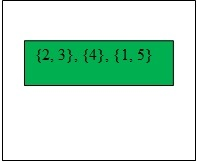
\includegraphics[width=30mm,scale=0.5]{Step1square.jpg}
\centering
\end{figure}
\item
Start with the top edge, and write a 1-cell that would be a face of the 2-cell.  
\begin{figure}[h] 
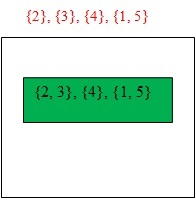
\includegraphics[width=30mm,scale=0.5]{Step2square.jpg}
\centering
\end{figure}
\item
Next, fill in the adjacent vertices, by referring to our list above.
\begin{enumerate}
\item 
The vertex that is always on the left of a particular face is all singletons, and in the same order as the 1-cell on that face. The vertex that always on the right is all singletons, in the same order as the 1-cell on the face, but the singletons that are paired will split in the opposite order. Thus, we get the top edge of the square, and the first face of the 2-cell.\\
\end{enumerate}
\begin{figure}[h] 
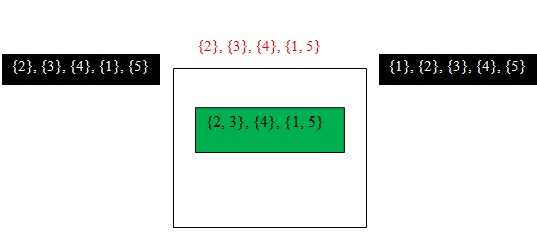
\includegraphics[width=70mm,scale=0.5]{Step3square.jpg}
\centering
\end{figure}
\item
Getting the other faces of the 2-cell
\begin{enumerate}
\item
By referring to our list above, we can look to see the vertices that the faces have in common,fill in the next face,then vertex, and eventually fill in the whole square.
For example, as we can see from our list,(\{2\},\{3\},\{4\},\{1,5\}) and (\{1\},\{2,3\},\{4\},\{5\}) have a vertex in common, so they should be next to each other, and the only vertex left for that face is (\{1\},\{3\},\{2\},\{4\},\{5\}), so that should be the next vertex.
\end{enumerate}
\begin{figure}[h] 
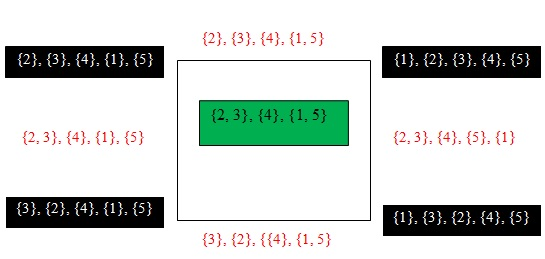
\includegraphics[width=70mm,scale=0.5]{Step5square.jpg}
\centering
\end{figure}
\item
Lastly, we write the orientation on the faces of the 2-cell. To determine orientation, we look at the face of the 2-cell and the vertices that are adjacent to that face.
\begin{enumerate}
\item
The arrow should be leaving the adjacent vertex to a particular edge that is all singletons, and is in the same order as the 1-cell on that face.
\item
The arrow should be pointing towards the vertex that is all singletons, in the same order as the 1-cell on the face, but the singletons that are paired will split in the opposite order.
\item
\begin{figure}[h] 
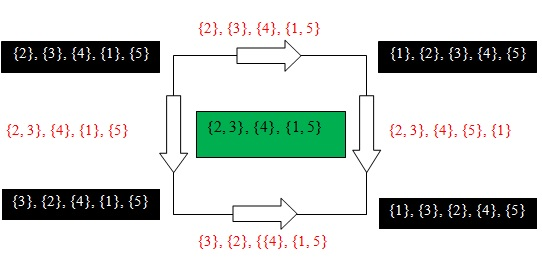
\includegraphics[width=70mm,scale=0.5]{Step6square.jpg}
\centering
\end{figure}
Note: This orientation, where the arrows on the left and right faces both point downwards, and the arrows on the top and bottom faces both point right will always be the same for 2-cells of this type.
\end{enumerate}
\end{enumerate}
\end{exmp}

Next, we will draw the second type of 2-cell, where we have a set with three entries and the other sets are just singletons.

The 2-cell we will be drawing is (\{1,2,3\},\{4\},\{5\} ), and we will still adhere to the rules about the orientation of the arrows in relation to the vertices and faces, as we did with the squares.
\begin{exmp} Drawing the second type of 2-cell.

Below, there is a list of all of the faces and their associated vertices. Again, we determined the faces of this 2-cell by the face relation,which is that we obtain faces of a cell by splitting one of its partite sets into $2$ nonempty parts \cite{}. In this case, a face would be a cell where $2$ out of the $3$ entries in the $3$ entry set are paired and the $3^{rd}$ entry is a singleton placed either on the right or left of this $2$ entries that are paired. Thus, there are $6$ possible faces and $6$ vertices.
\begin{enumerate}
\item
(\{1,2\},\{3\},\{4\},\{5\})
\begin{itemize}
\item 
(\{1\},\{2\},\{3\},\{4\},\{5\})
\item
(\{2\},\{1\},\{3\},\{4\},\{5\})
\end{itemize}
\item
(\{3\},\{1,2\},\{4\},\{5\})
\begin{itemize}
\item
(\{3\},\{1\},\{2\},\{4\},\{5\})
\item
(\{3\},\{2\},\{1\},\{4\},\{5\})
\end{itemize}
\item
(\{2,3\},\{1\},\{4\},\{5\})
\begin{itemize}
\item 
(\{2\},\{3\},\{1\},\{4\},\{5\})
\item
(\{3\},\{2\},\{1\},\{4\},\{5\})
\end{itemize}
\item
(\{1\},\{2,3\},\{4\},\{5\})
\begin{itemize}
\item 
(\{1\},\{2\},\{3\},\{4\},\{5\})
\item
(\{1\},\{3\},\{2\},\{4\},\{5\})
\end{itemize}
\item
(\{1,3\},\{2\},\{4\},\{5\})
\begin{itemize}
\item 
(\{1\},\{3\},\{2\},\{4\},\{5\})
\item
(\{3\},\{1\},\{2\},\{4\},\{5\})
\end{itemize}
\item
(\{2\},\{1,3\},\{4\},\{5\})
\begin{itemize}
\item 
(\{2\},\{1\},\{3\},\{4\},\{5\})
\item
(\{2\},\{3\},\{1\},\{4\},\{5\})
\end{itemize}
\end{enumerate}
\begin{enumerate}
\item
Draw a hexagon, start at the top edge with a face of the 2-cell.
\begin{figure}[htb!]
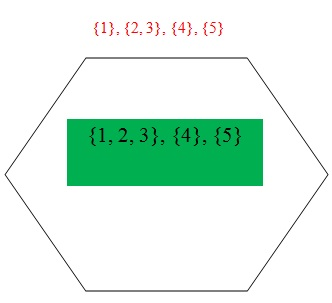
\includegraphics[width=40mm,scale=0.5]{Step1hexagon.jpg}
\centering
\end{figure}
\item
Next, write in the adjacent vertices on the top edge, using our rule from drawing the squares and referring to the list above. 
\begin{figure}[htb!]
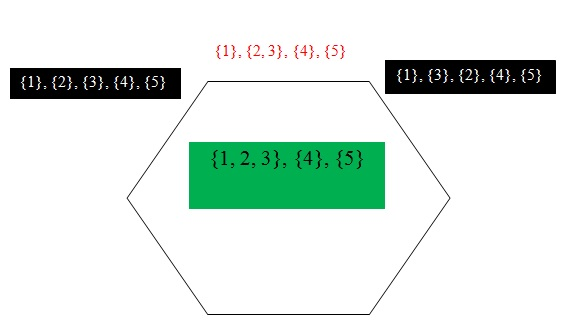
\includegraphics[width=70mm,scale=0.5]{Step2hexagon2.jpg}
\centering
\end{figure}
\item
Finishing the hexagon:

Start from the top right edge and go around the hexagon. By referring to our list above, we can look to see the vertices that the faces have in common,fill in the next face,then vertex, and eventually fill in the whole hexagon.
For example, as we can see from our list,(\{1\},\{2,3\},\{4\},\{5\}) and (\{1,3\},\{2\},\{4\},\{5\}) have a vertex in common, so they should be next to each other, and the only vertex left for that face is (\{3\},\{1\},\{2\},\{4\},\{5\}), so that should be the next vertex.
\begin{figure}[htb!]
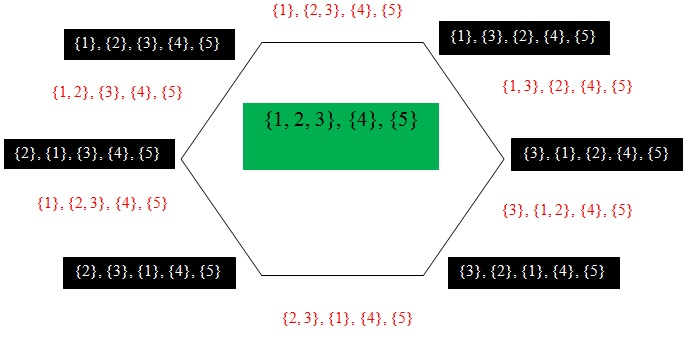
\includegraphics[width=70mm,scale=0.5]{Step4hexagon.jpg}
\centering
\end{figure}
\item
Lastly, we would place arrows on the edges of the hexagon based on orientation, as we did for the squares.
\end{enumerate}
\begin{figure}[htb!] 
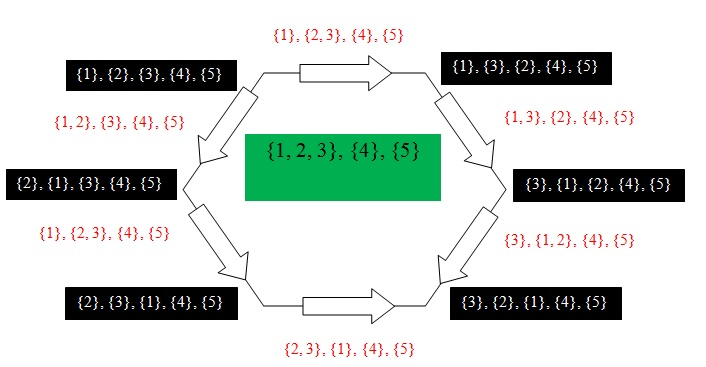
\includegraphics[width=70mm,scale=0.5]{Step5hexagon.jpg}
\centering
\end{figure}
\end{exmp}
\subsection{Discrete Morse Theory}
\begin{definition} \cite{RFOR}
A \textit{discrete vector field} is a map
\begin{equation}
W: K \rightarrow K \cup \{0\}
\end{equation}
satisfying 
\begin{enumerate}
\item for each $ p, W(K_p) \subseteq K_{(p+1)} \cup \{0\}$
\item for each $\sigma^p$ $\in K_p$, either $W(\sigma) = 0$ or $\sigma$ is a regular face of $W(\sigma)$ 
\item if $\sigma$ $\in$ Image($W$) then $W(\sigma) = 0$
\item for each $\sigma^p \in K_p$ 
\end{enumerate}
\begin{equation}
\# \{v^{p-1} \in K_{p-1}  |  W(v) = \sigma\} \leq 1
\end{equation}
\end{definition}

\begin{definition} \cite{RFOR}
Let $W$ be a combinatorial vector field. A $W$-\textit{path of dimension p} is a sequence of p-cells
\begin{center}
$\gamma = \sigma_1, \sigma_1, ..., \sigma_r$
\end{center}
such that
\begin{enumerate}
\item if $W(\sigma_i) = 0$ then $\sigma_{i+1} = \sigma_i$
\item if $W(\sigma_i) \neq 0$ then $\sigma_{i+1} \neq \sigma_i$ and $\sigma_{1+1} <W(\sigma_i)$ 
\end{enumerate}
say $\gamma$ is a \textit{closed path} if $\sigma_r = \sigma_0$ and $\gamma$ is \textit{non-stationary} if $\sigma_1$ $\neq \sigma_0$. 
\end{definition}
\begin{theorem}
Let $W$ be a discrete vector field. There is a discrete Morse
function $f$ with $W=V_f$ if and only if $W$ has no non-stationary closed paths. Moreover, for every such $W$, $f$ can be chosen to have the property that if
$\sigma^{p}$ is critical, then
\begin{center}
$f({\sigma})=p$
\end{center}
Such a Morse function is said to be self-indexing.
\end{theorem}

\begin{remark} 
Note that $W$ determines the critical points of $f$. Namely, if
$W=V_{f}$, then, by the lemma 6.3, $\sigma\in K_p$ is critical for $f$ if and only if $W(\sigma)=0$ and $ \sigma\not\in Image(W)$.
\end{remark}

\begin{definition}
Let $W$ be a discrete vector field on $X$. A \textit{W-path of dimension $p$} is a sequence of $p$-cells $\sigma_0, \sigma_1, . . . , \sigma_r$ such that if $W(\sigma_i)$ is undefined, then $\sigma_{i+1} = \sigma_i$ , and otherwise $\sigma_{i+1} \neq \sigma_i$ and $\sigma_{i+1} < W(\sigma_i)$. The W-path is closed if $\sigma_r = \sigma_0$, and \textit{non-stationary} if $\sigma_1 \neq \sigma_0$. A discrete vector field $W$ is a \textit{discrete gradient vector field} if $W$ has no non-stationary closed paths.
\end{definition}

\begin{definition}
Given any discrete gradient vector field $W$ on $X$, there is an associated classification of cells in $X$ into 3 types: redundant, collapsible, and critical (this terminology is partially borrowed from [12] as well as from Ken Brown, [7]).
A cell $\sigma \in K$ is \textit{redundant} if $\sigma \in $ domW, \textit{collapsible} if $\sigma \in$ imW, and \text{critical} otherwise. The \textit{rank} of a cell $c$ with respect to a discrete gradient vector
field $W$ is the length of the longest $W$-path $c = c_1, . . . , c_r$ having the property that $c_i \neq c_j$ if $i \neq j$. Critical and collapsible cells all have rank 1, and redundant cells are of rank at least 2. If $c^{\prime} < W(c)$ and $c \neq c^{\prime}$ , then clearly $rank(c^{\prime}) < rank(c)$.
\end{definition}

\begin{definition}
An \textit{alphabet} is simply a set $\sum$. The \textit{free monoid} on $\sum$, denoted $\sum^*$ , is the
collection of all positive words in the generators $\sum$, together with the empty
word, endowed with the operation of concatenation.
\end{definition}

\begin{definition}
A \textit{monoid presentation} denoted $\langle \sum | R \rangle$, consists of an alphabet $\sum$ together
with a collection $R$ of ordered pairs of elements in $\sum^*$ . An element of $R$ should
be regarded as an equality between words in $\sum^*$, but, in what follows, the order
will matter.
\end{definition}

\begin{definition}
A \textit{rewrite system} $\Gamma$ is an oriented graph. The vertices of $\Gamma$ are called \textit{objects} and
the positive edges are called \textit{moves}. If $v_1$ is the initial vertex of some positive
edge in $\Gamma$ and $v_2$ is the terminal vertex, then write $v_1 \rightarrow _\Gamma \thinspace v_2 $ or $v_1 \rightarrow v_2$ if
the name of the specific rewrite system is clear from the context. An object is
called \textit{reduced} if it is not the initial vertex of any positive edge (move). The
reflexive, transitive closure of $\rightarrow$ is denoted $\dot{\rightarrow}$ .
\end{definition}

\begin{definition}
Every monoid presentation $\langle\sum | R \rangle $ has a natural rewrite system, called a \textit{string
rewriting system}, associated to it. The set of objects of this string rewriting
system is the free monoid $\sum ^*$ . There is a move from $w_1 \in \sum^*$ to $w_2 \in  \sum^*$ if
$w_1 = ur_1v$ and $w_2 = ur_2v$ in $\sum^*$ , where u, v $\in \sum^*, (r_1, r_2) \in R$.
\end{definition}

\begin{proposition}
\begin{enumerate}
\item The inclusion of $X^\prime_n$ into $X$ induces an isomorphism from $\pi_{n-1}(X^\prime_n)$ to $\pi_{n-1}(X)$.
\item If $X$ has no critical cells of dimension greater than $k$, then $X \searrow X^\prime_k$ .
\item $X$ is homotopy equivalent to a CW complex with $m_n$
cells of dimension $n$, where $m_n$ is the number of critical n-cells in $X$.
\item The subcomplex of $X$ generated by the collapsible and critical edges is connected.
\item The subcomplex of $X$ generated by the collapsible edges and the 0- skeleton of $X$ is a maximal forest.
\item If there is only one critical 0-cell, then the graph consisting of (the closures of) the collapsible edges is a maximal tree in $X$.
\end{enumerate}

\end{proposition}

\begin{subsubsection} {Monoid Presentation}
Choose a maximal tree $T$ of $X$ consisting of all of the collapsible edges in $X$, and additional critical edges, as needed.\\
Define a monoid presentation $MP_{W,T}$ as follows: Generators are oriented edges in $X$, both positive and negative, so that there are two oriented edges for each geometric edge in $X$. If $e$ denotes a particular oriented edge, let $\overline{e}$ denote the edge with the opposite orientation. If $w$ denotes a sequence of oriented edges $e_1 . . . e_m$, let $\overline{w}$ denote sequence of oriented edges $\overline{e_m} . . . \overline{e_1}$ .

\begin{definition}
A \textit{boundary word} of a 2-cell $c$ is simply one of the possible relations determined
by an attaching map for $c$ (cf. [19], page 139); if $w_1$ and $w_2$ are two boundary words for a cell $c$, then $w_1$ can be obtained from $w_2$ by the operations of inverting and taking cyclic shifts. 
\end{definition}
There are several types of relations.
\begin{enumerate}
\item For a given oriented edge $e$ in $T$ , introduce the relations $(e, 1)$ and $(\overline{e}, 1)$.
\item For any oriented edge $e$, introduce relations $(e\overline{e}, 1)$ and $(\overline{e}e, 1)$.
\item For a collapsible 2-cell $c$, consider the (unique) geometric 1-cell $e$ such that $e = W^{-1}(c)$. Suppose that a boundary word of $c$ is $ew$. In this case, the word $w$ contains no occurrence of $e$ or $\overline{e}$, since the geometric edge corresponding to $e$ is a regular face of $c$. Introduce the relations
$(e,\overline{w})$ and $(\overline{e},w)$.
\end{enumerate}
\begin{proposition}
The rewrite system associated to the monoid presentation
$MP_{W,T}$ is complete.
\end{proposition}

In view of Proposition [], there is a unique reduced word in each equivalence class modulo the presentation $MP_{W,T}$. If $w$ is any word in the generators of $MP_{W,T}$ , let $r(w)$ denote the unique reduced word that is equivalent to $w$. 
\end{subsubsection}

\begin{theorem} 
Let $X$ be a finite connected $CW$ complex with a discrete gradient vector field $W$. Then:
\begin{equation}
\pi_1(X) \cong \langle \Sigma | R \rangle,
\end{equation}
where $\sum$ is the set of positive critical 1-cells that are not contained in $T$ , and
R = \{$r(w)|w$ is the boundary word of a critical 2-cell\}.
\end{theorem}

In case there is just one critical 0-cell, the discrete gradient vector field $W$ completely determines the maximal tree $T$ , and we denote the presentation $\langle \Sigma | R \rangle$ from the previous theorem $P_W$ , where the oriented CW complex is understood. The presentation $P_W$ depends only on the choice of the boundary words for the critical 2-cells, since the string rewriting system associated to the monoid presentation $MP_{W,T}$ is complete and by the previous theorem.


\subsection{Discrete Gradient Vector Field on M(L)}

\begin{definition}\cite{PANZU} A \textit{discrete vector field} is a set of pairs ($\alpha^{p}$, $\beta^{p+1}$)
such that:
each cell of the complex participates in at most one pair, and\\
in each pair, the cell $\alpha^{p}$,  is a facet of $\beta^{p+1}$.
\end{definition}

Below we describe a discrete gradient vector field.
According to the definition, we introduce some pairings of the cells.\\
\textbf{Step 1.} We pair together\\
\begin{center}
{$\alpha$ = (... \{1\} \textit{I} ...) and $\beta$ = (... \{1\} $\cup$ \textit{I}...)}
\end{center}
iff the following holds:\\
\begin{enumerate}
\item the set \textit{I} does not contain \textit{n}, and
\item the set \{1\} $\cup$ \textit{I} is short.
\end{enumerate}

Before we pass to step 2, observe that the non-paired cells are labeled by one of the following types of labels:
\begin{center}
(... \{1,*,$n$\})
\end{center}
\begin{center}
(... \{1\} \{*,$n$\})
\end{center}
\begin{center}
(... \{1\} (a 1-prelong set)...)
\end{center}

\textbf{Step 2.} We pair together
\begin{center}
$\alpha$ = (... \{2\} \textit{I}...) and $\beta$ = (... \{2\} $\cup$ \textit{I}...)
\end{center}
iff the following holds:
\begin{enumerate}
\item The set I contains neither \textit{n}, nor 1.
\item The set \{2\} $\cup$ \textit{I} is short.
\item $\alpha$ and $\beta$ were not paired at the previous step.
\end{enumerate}
After this step, the non-paired cells are labeled by one of the following types of labels: 

\begin{center}
(...,1,2,*,\{\textit{n}\})
\end{center}

\begin{center}
(...,\{1\}\{2,*,\textit{n}\})
\end{center}

\begin{center}
(...,\{2\}\{1,*,\textit{n}\})
\end{center}

\begin{center}
(...,\{2\}\{1\}\{*,\textit{n}\})
\end{center}

\begin{center}
(...,\{2\} \{1\}(a 1-prelong set)...)
\end{center}

\begin{center}
(...,\{1\} (a 1-prelong set)... \{2\}\{*,\textit{n}\})
\end{center}

\begin{center}
(...,\{2\} (a 2-prelong set not containing 1)... \{1\}\{*,\textit{n}\})
\end{center}

\begin{center}
(...,\{1\} (a 1-prelong set not containing 2)... \{2,*,\textit{n}\})
\end{center}

\begin{center}
(...,\{2\} (a 2-prelong set not containing 1)... \{1,*,\textit{n}\})
\end{center}

We proceed this way for all k \textless \textit{n}, assuming that the step number k looks
as follows:

\textbf{Step k.} We pair together\\
\begin{center}
$\alpha$ = (... \{k\} \textit{I}...) and $\beta$ = (...\{k\} $\cup$ \textit{I}...)
\end{center}

iff the following holds: 
\begin{enumerate}
\item The set \textit{I} contains none of \textit{n}, 1, 2, ..., k-1.
\item The set \{k\} $\cup$ \textit{I} is short.
\item $\alpha$ and $\beta$ were not paired at the previous steps.
\end{enumerate}
We proceed pairing for all k = 1, 2, ..., n-1.

\begin{definition}
\cite{PANZU} An entry \textit{k} is \textit{forward-movable} (with respect to the cell $\alpha$), if it forms a singleton, which followed by a set \textit{I}, \textit{n} $\not\in$ \textit{I} such that
\begin{enumerate}
\item {\textit{k} \textless \textit{i} for every $\textit{i}$ $\in$ \textit{I}, and}
\item{\{\textit{k}\} $\cup$ \textit{I} is short.}
\end{enumerate}
\end{definition}

\begin{example} 
Suppose \textit{n}=7\\
\begin{enumerate}
\item Say we have a $0$-cell: (\{2\}, \{1\}, \{3\}, \{6\}, \{5\}, \{4\},\{7\}) where L= \{1,1,1,2,4,5,5\}.\\
First we will join \{1\} with \textit{I}. In this particular case \textit{I} is \{3\}. Since \{1,3\} is short (\{2\}, \{1\}, \{3\}, \{6\}, \{5\}, \{4\},\{7\}) is forward movable since it is in the domain. 

\item \textbf{Non-example:} The 1-cell: (\{6\}, \{4\}, \{3\}, \{2\}, \{1\}, \{5,7\}) is not forward movable because \{1\} cannot join with \textit{I}. Since \{1\} cannot join with \textit{I} we move onto \{2\}. Because \{2\} cannot join with \textit{I} we move onto \textit{\{k\}}. Therefore, (\{6\}, \{4\}, \{3\}, \{2\}, \{1\}, \{5,7\}) is not forward-movable.       
\end{enumerate}
\end{example}

\begin{definition}
\cite{PANZU} An entry \textit{k} is \textit{backward-movable} if the following holds:
\begin{enumerate}
\item 
{entry \textit{k} lies in a non-singleton set J, \textit{n} $\not\in$ J;}
\item 
{\textit{k}=$\min(J)$;}

\item
{one of the following conditions hold:}
\begin{enumerate}
\item the set J is preceded by a non-singleton set;
\item the set J is preceded by a singleton \{\textit{m}\} with \textit{m} $>$ k;
\item the set J is preceded by the \textit{n}-set.
\end{enumerate}
\end{enumerate}
\end{definition}

\begin{example} Suppose \textit{n}=7
\begin{enumerate}
\item Say we have a 1-cell: (\{5\}, \{2\}, \{1,3\}, \{4\}, \{6\}, \{7\}) where L= \{1,1,1,2,4,5,5\}. Note that we have an entry \textit{k} that lies in a non-singleton set J, \textit{n} $\not\in$ J. Since \textit{k} = $\min$(J) then 1 is backward-movable. 
\\Note that this 1-cell came from (\{5\}, \{2\}, \{1\}, \{3\}, \{4\}, \{6\}, \{7\}).
\item \textbf{Non-Example:}
In the 1-cell (\{2\}, \{4\}, \{3\}, \{5\}, \{6\}, \{1,7\}) \textit{K} does not lie in a non-singleton set J, \textit{n} $\not\in$ J. Therefore, it is not backward-movable. 
\item \textbf{Non-Example:}
In the 1-cell (\{3\}, \{2,4\}, \{1\}, \{6\}, \{5\}, \{7\}) \textit{k} lies in a non-singleton set \textit{J}, \textit{n} $\not\in$ \textit{J}. In this case \textit{k}=2 and $k = \min{J}.$ But \textit{J} is not preceded by a non-singleton set. Nor does it satisfy that the set J is preceded by a singleton \{m\} with $m>k$; or that the set \textit{J} is preceded by the \textit{n}-set. Therefore \text{k} is not backward-movable.\\
Note that the 1-cell is forward-movable since \{1\} can join with \{6\} making it (\{3\}, \{2,4\}, \{1,6\}, \{5\}, \{7\}). 
\end{enumerate}
\end{example}

\begin{definition}
\cite{PANZU}\textit{Critical cells} are the cells that are non-paired. They are exactly those with empty set of movable entries.
\end{definition}

\textbf{Notation}: 
\begin{enumerate}
\item By "\ldots " we denote any ordered admissible collection of subsets of [n],which as well can be the empty set.
\item By ''*''we denote any subset of [n], which as well can be the empty set.
\item A set I $\subset$ [n] is \textit{k-prelong}, if I is short, and I $\cup$ \{k\} is long.
\item For a set $I \cup [n]$ and an entry $k \in [n]$, we write $k  < I$ whenever $\forall i \in I$,  $k < i$. 
\item Analogously, we write $k=min(I)$ whenever k is the minimal entry of the set I.
\item Unlike "...", by "$\varheartsuit$" and "$\Diamondblack$" we denote a (possibly empty) string of singletons going in the decreasing order. For instance, "$\Diamondblack$" can be (\{7\}, \{4\}, \{2\}), but can be neither (\{7,4,2\} nor (\{4\}, \{2\}, \{7\}).
\end{enumerate} 


\begin{theorem}\cite{PANZU}
The critical cells of the introduced above discrete Morse function are exactly all cells of the two following types.
\end{theorem}

\textbf{Type 1.}
\begin{center}
($\varheartsuit$ \{*, \textit{n}\}).
\end{center}

\textbf{Example:}
\begin{enumerate}
\item \ $\{\{6\},\{5\},\{4\},\{2\},\{1\},\{3,7\}\}$ is an example of a critical 1-cell.
\item$\{\{6\},\{5\},\{4\},\{1\},\{2,3,7\}\}$ is an example of a critical 2-cell.
\end{enumerate}
\textbf{Type 2.}\\
\indent\indent($\varheartsuit$ \{ \textit{k}\} \textit{I} $\Diamondblack$ \{ \textit{n},*\}), if the following conditions hold: 
\begin{enumerate}
\item \textit{I} is a \textit{k}-prelong set not containing \textit{n}.
\item \textit{k} $<$ \textit{I}
\item \textit{k} $<$ $\varheartsuit$\\
(In other words, ($\varheartsuit$ \{\textit{k}\}) is an ordered string of singletons.)
\end{enumerate}
\textbf{Example:} Suppose n=7 where L= \{1,1,1,2,4,5,5\}.\\
Say we have the 2-cell $\{\{3\},\{5,6\},\{4\},\{2\},\{1,7\}\}$. In this case, \textit{k}=\{3\}. k $\cup$ I is k-prelong and $k<I$ therefore $\{\{3\},\{5,6\},\{4\},\{2\},\{1,7\}\}$ is an example of a critical 2-cell.  \\
\section{Our Research}

\begin{definition}
Let $e$ be a $1$-cell in M(L). We define $p(e)$ as follows:
\begin{enumerate}
\item If $m$ is neither forward nor backward-movable $\forall m\in \{1,\ldots,n\}$, then $p(e)=e$.
\item If $m$ is the smallest movable entry and is backward-movable, then $p(e)=1$.
\item If $m$ is the smallest movable entry and is forward-movable, then $e=(\ldots,\{m\},I,\ldots)$ and we define $p(e)=(\ldots,I,\{m\},\ldots)$.
\end{enumerate}
\end{definition}

\begin{remark}
We define $p(\overline{e})=\overline{p(e)}$.
\end{remark}

\begin{example}
Continuing to use the equilateral heptagon from the previous examples, the following statements hold:
\begin{enumerate}
\item Let $e=(6,5,4,2,3,\{1,7\})$, then $p(e)=(6,5,4,3,2,\{1,7\})$.
\item Let $e=(\{4,6\},5,3,2,1,7)$, then $p(e)=1$.
\item Let $e=(2,4,6,5,1,\{3,7\}$, then $p(e)=(4,2,6,5,1,\{3,7\})$.
\end{enumerate}
\end{example}

\begin{definition}
Given a redundant 1-cell $e=(\ldots,\{k\},\{l\},\ldots,\{m,n\})$, where k is the smallest forward-movable integer, we define $q(e)$ such that $q(e)=(\{m\},\ldots,\{k,l\},\ldots,\{n\})$.
\end{definition}

\begin{example}
Given $e=(4,6,2,3,5,\{1,7\})$, $q(e)=(1,4,6,\{2,3\},5,7)$.
\end{example}

\begin{definition}
For a 1-cell $e$, there is $m\in\bn$ such that $p^{m}(e)=1$ or $p^{m}(e)=p^{m+1}(e)$. We define $p^{\infty}(e)=p^{m}(e)$.
\end{definition}

\begin{example}
In reference to the same heptagon that we have been using in the previous examples, we can conclude the following:
\begin{enumerate}
\item If $e=(1,2,\{3,4\},5,6,7)$, then $p^{\infty}(e)=1$.
\item If $e=(3,2,4,1,6,\{5,7\})$, then $p^{\infty}(e)=(6,4,3,2,1,\{5,7\})$.
\end{enumerate}
\end{example}

\begin{theorem}
If $e$ is a 1-cell such that n is the only element in the n-set, then $r(e)=p^{\infty}(e)$. 
\end{theorem}

\begin{proof}
%Add something like, "We first show that"
$r(e)$ follows the discrete gradient vector field, i.e. $p(e)$ uses the boundary map of $v_{1}(e)$ to rewrite $e$.
\begin{enumerate}
\item Case I: ($I$ is a singleton) In this case $e$ flows into a 2-cell, (\ldots,\{m,k\},\ldots,\{i,j\},\ldots,n), which is in the shape of a square (as demonstrated \textbf{Section 2.2}). The edge $e$ can be rewritten using the boundary of the rest of the square: $e_{l}e_{b}\overline{e_{r}}$ (l=left, b=bottom, r=right). For $e_{l}$ and $e_{r}$ the smallest unstuck integer, $m$, is in a pair because that is what flowing across the 2-cell represents. However, $m$ is a collapser and so both $e_{l}=1$ and $e_{r}=1$. Therefore $r(e)=e_{b}=p(e)$ which is either the identity (if $i$ is a collapser) or $e=p(e_{b})$.
\item Case II: ($I$ is a pair) In this case $e$ flows into a 2-cell, (\ldots,\{m,i,j\},\ldots,n), which is in the shape of a hexagon. So $e$ can be rewritten as $e_{1}e_{2}e_{3}\overline{e_{4}e_{5}}$ (sides 1\ldots5 are obtained by tracing the hexagon counterclockwise). The sides $e_{1},e_{2},\overline{e_{4}}$ and $\overline{e_{5}}$ all include the pairs \{m,i\} or \{m,j\},
making all those sides equal the identity (since $m$ is a collapser). Therefore $r(e)=e_{3}=p(e)$ and either $e_{3}=1$ if $i$ is a collapser, or $e_{3}=p(e_{3})$.
\end{enumerate}
Since $v_{1}$ is an injective function, $r$ is vacuously confluent.
%I actually think this needs more explanation now, I also don't think we care about injectivity for confluent. Maybe add, "Since $v_1$ is a function, p(e) has a unique output, so $r(e)$ is unique and is therefor confluent" I hate to say it but maybe talking about the dgvf wasn't the way to go? I think you should probably discuss with Farley soon, I can be there too if you want.
Also because $r$ follows a discrete gradient vector field, it cannot flow to non-stationary closed paths, and terminates. Therefore this rewriting system is complete and $p^{\infty}(e)$ represents a finite flow over the discrete gradient vector field.
\end{proof}

\begin{theorem}
If $e=(\ldots,\{m,n\})$, where the n-set has exactly 2 elements, then
\begin{enumerate}
\item $e\dot{\rightarrow}p(e)$, if $e$ is critical or the smallest forward-movable integer is less than m,
\item $e\dot{\rightarrow}p(e)\overline{q(e)}$ otherwise.
\end{enumerate}
$r(e)$ can be computed by continuously applying this procedure.
\end{theorem}

\begin{proof}
\noindent
\begin{enumerate}
\item The same proof applies here as that of \textbf{Theorem 3.11}. %explain why the same proof applies
\item The 2-cell that $e$ flows into is (\ldots,\{k,l\},\ldots,\{m,n\}). So if e were to be rewritten using the boundary of the 2-cell $e=e_{l}e_{b}\overline{e_{r}}$. We can see that $e_{l}=1$ because after the repeated application of $p^{\infty}(e_{l})$ the integer $k$ becomes a collapser. Also observe that $e_{b}=p(e)$ and  $\overline{e_{r}}=\overline{q(e)}$. Thus $r(e)=p(e)\overline{q(e)}=s(e)$ which,
%$r(e)=p(e)\overline{q(e)}=s(e)$ is not right, I think you want something like $\partial (v_1(e))= e_{l}p(e)\overline{q(e)}  and e_l is pre-collapsable?  or maybe just $s(e)=p(e) \overline{q(e)}$, get rid of the r(e)
follows the discrete gradient vector field so, is again confluent and terminates.
\end{enumerate}
\end{proof}

\begin{theorem}
If a critical 2-cell is of the form ($\Diamondblack$,\{a,b,n\}),then the generators ($\Diamondblack$,\{a,n\})\\
and ($\Diamondblack$,\{b,n\}) commute.
\end{theorem}

\begin{proof}
Starting with the 2-cell of the form $(\Diamondblack,\{a,b,n\})$, the boundary gives the relation:
\begin{equation*}
(\Diamondblack,a,bn)(\Diamondblack,an,b)(\Diamondblack,n,ab)\overline{(\Diamondblack,bn,a)(\Diamondblack,b,an)(\Diamondblack,ab,n)}=1.
\end{equation*}
This simplifies to:
\begin{equation*}
(\Diamondblack,bn)(\Diamondblack,an)(\Diamondblack,n,ab)\overline{(\Diamondblack,bn)(\Diamondblack,an)(\Diamondblack,ab,n)}=1.
\end{equation*}
Since $a$ is a backward-movable, $(\Diamondblack,n,ab)$ and $\overline{\Diamondblack,ab,n}$ both go to the identity, and we are left with the relation:
%See how the a,b,n look different outside of equation mode? jsyk this is why cells need to be in math mode
\begin{equation*}
(\Diamondblack,bn)(\Diamondblack,an)\overline{(\Diamondblack,bn)(\Diamondblack,an)}=1.
\end{equation*}
\end{proof}

\begin{theorem}
If a critical 2-cell is of the form ($\varheartsuit$,\{r,q\},$\Diamondblack$,\{a,n\}), then the critical 1-cells ($\varheartsuit$,\{r,q\},$\Diamondblack$,n) and ($\Diamondblack$,\{a,n\}) commute.
\end{theorem}

\begin{proof}
Starting with the 2-cell of the form ($\varheartsuit$,\{r,q\},$\Diamondblack$,\{a,n\}), the boundary give the relation:
\begin{equation*}
(\varheartsuit,r,q,\Diamondblack,\{a,n\})(a,\varheartsuit,\{r,q\},\Diamondblack,n)\overline{(\varheartsuit,q,r,\Diamondblack,\{a,n\})(\varheartsuit,\{r,q\},\Diamondblack,a,n)}=1.
\end{equation*}
Applying $p^{\infty}(x)$ to each edge:
%You are just applying $P^{\infty} to each edge, don't need "(x)" to represent function
\begin{equation*}
(\Diamondblack,\{a,n\})(\varheartsuit,\{r,q\},\Diamondblack,n)\overline{(\Diamondblack,\{a,n\})(\varheartsuit,\{r,q\},\Diamondblack,n)}=1.
\end{equation*}
\end{proof}

\begin{corollary}
Assume that $\{n-3, n-2, n-1\}$ is short. Let $I = \{ i \in \{1,\ldots, n-1\} \mid \{i,n\}$ is short\}; let $J = \{ \{j,k\} \subseteq \{1,\ldots, n-1\} \mid \{j,k,n\}$ is short\}.
\[ \pi_{1}(X)\cong\langle x_i \, (i \in I): [x_{j}, x_{k}] \, (\{j,k\}\in J) \rangle. \]
\end{corollary}

\begin{proof}
Let $X$ be a moduli space with a regular cell complex. By assumption, since \{n-3,n-2,n-1\} is short, there are no long 3-element sets (not including the n-sets). Therefore critical 2-cells of Type II cannot exist, leaving critical 2-cells of Type I. By \textbf{Theorem 3.13} there are $\dbinom{n-1}{2}$ Type I critical 2-cells withis $\dbinom{n-1}{n-2}=n-1$ critical 1-cells. This means that there are $n-1$ generators and they commute.
% It's not quite enough to just count the relations, some could appear more than once. You need to justify why you get a commutor for each pair of generators (This is because for each choice of $i,j$, $(\Diamondblack, {i,j,n})$ isa  critical 2-cell)

\end{proof}

\begin{corollary}
If \{n-2,n-1\} is long, then $\pi_{1}(X)\cong\bz^{n-3}$.
\end{corollary}

\begin{proof}
Let $X$ be a moduli space with a regular cell complex. Since \{n-2,n-1\} is long, $X$ is disconnected and any 2-cell of type (\ldots,\{l,k\},\ldots,\{m,n\}) is always collapsible. This is because there will always be a collapser in the pair that is not the n-set. Therefore there are only Type II critical 2-cells of the form ($\Diamondblack$,\{a,b,n\}) or (n-2,n-1,$\Diamondblack$,\{a,b,n\}). Since \{n-2,n-1\} is long, so are \{n-1,n\} and \{n-2,n\}. Thus the only critical 1-cells are of the form ($\Diamondblack$,\{v,n\}) such that $v\leq n-3$. So there are $n-3$ generators, and as a result of \textbf{Theorem 3.13} they all commute.

%Again, just need to say that every $(\Diamondblack,\{a,b,n\})$ cell exists
\end{proof}



%Comments: 
%Variables should always be in math mode, including the n in $n$-set and $\{m\}$
% numbers should either be in math mode or spelled out depending on context. i.e. The set $\{n-2,n-1\}$ is short vs. there are two cases 

\textbf{Acknowledgements.} Firstly, we would like to thank Dr. Dan Farley for assisting us throughout the program, from "translating" difficult concepts to developing our research, his guidance was greatly appreciated. Also, for her continuous dedication and support, we would like to thank Hannah Hoganson, our graduate assistant, for always "un-complicating" the complicated. The opportunity SUMSRI has given us to explore undergraduate research in mathematics is one that has been crucial for our mathematical maturity, and for that we would like to thank all the staff and faculty that were involved. We would also like to thank Miami University for providing us with funds, housing and a place to learn and develop our research. Lastly, we thank the National Security Agency for funding this research program and making all this possible.


\newpage
%Bibliographic references
\begin{thebibliography}{4}

\bibitem{FS1} 
Daniel Farley and Lucas Sabalka. 
\textit{Discrete Morse Theory and graph braid groups}. 
Algebraic and Geometric Topology, 5(3):1079-1085, 2005.

\bibitem{RFOR} 
Robin Forman. 
\textit{Morse theory for cell complexes}. 
Advances in Mathematics, 134(1):90-145, 1998.

\bibitem{KAPMIL} 
Michael Kapovich and John Millson. 
\textit{On the Moduli Space of Polygons in the Euclidean plane}. 
Journal of Differential Geometry, 42(1):133-164, 1995.

\bibitem{PANZU} 
Gaiane Panina and Alena Zhukova. 
\textit{Discrete Morse theory for Moduli Spaces of Flexible Polygons, or Solitaire Game on the Circle}. 
ArXiv e-prints, 2015.

\end{thebibliography}

\end{document}








